\section{Requirement 4: slightly non-stationary multiple-campaigns environment}

% ============================================================
% Overview
% ============================================================
\begin{frame}{Slightly non-stationary multiple-campaigns environment}
    \begin{itemize}
        \item Rounds partitioned in \emph{stationary intervals} (phases), each with its own joint distribution of highest competing bids $m_p^{(i)}$
        \item Algorithms to be compared:
        \begin{itemize}
            \item \textbf{Combinatorial-UCB with sliding window}
            \item \textbf{Combinatorial-UCB with CUSUM change detection}
            \item \textbf{Primal-dual} (same as Req 3, no change awareness)
        \end{itemize}
    \end{itemize}
\end{frame}

% ============================================================
% Distribution model
% ============================================================
\begin{frame}{Distribution model: piecewise-stationary phases}
    \centering
    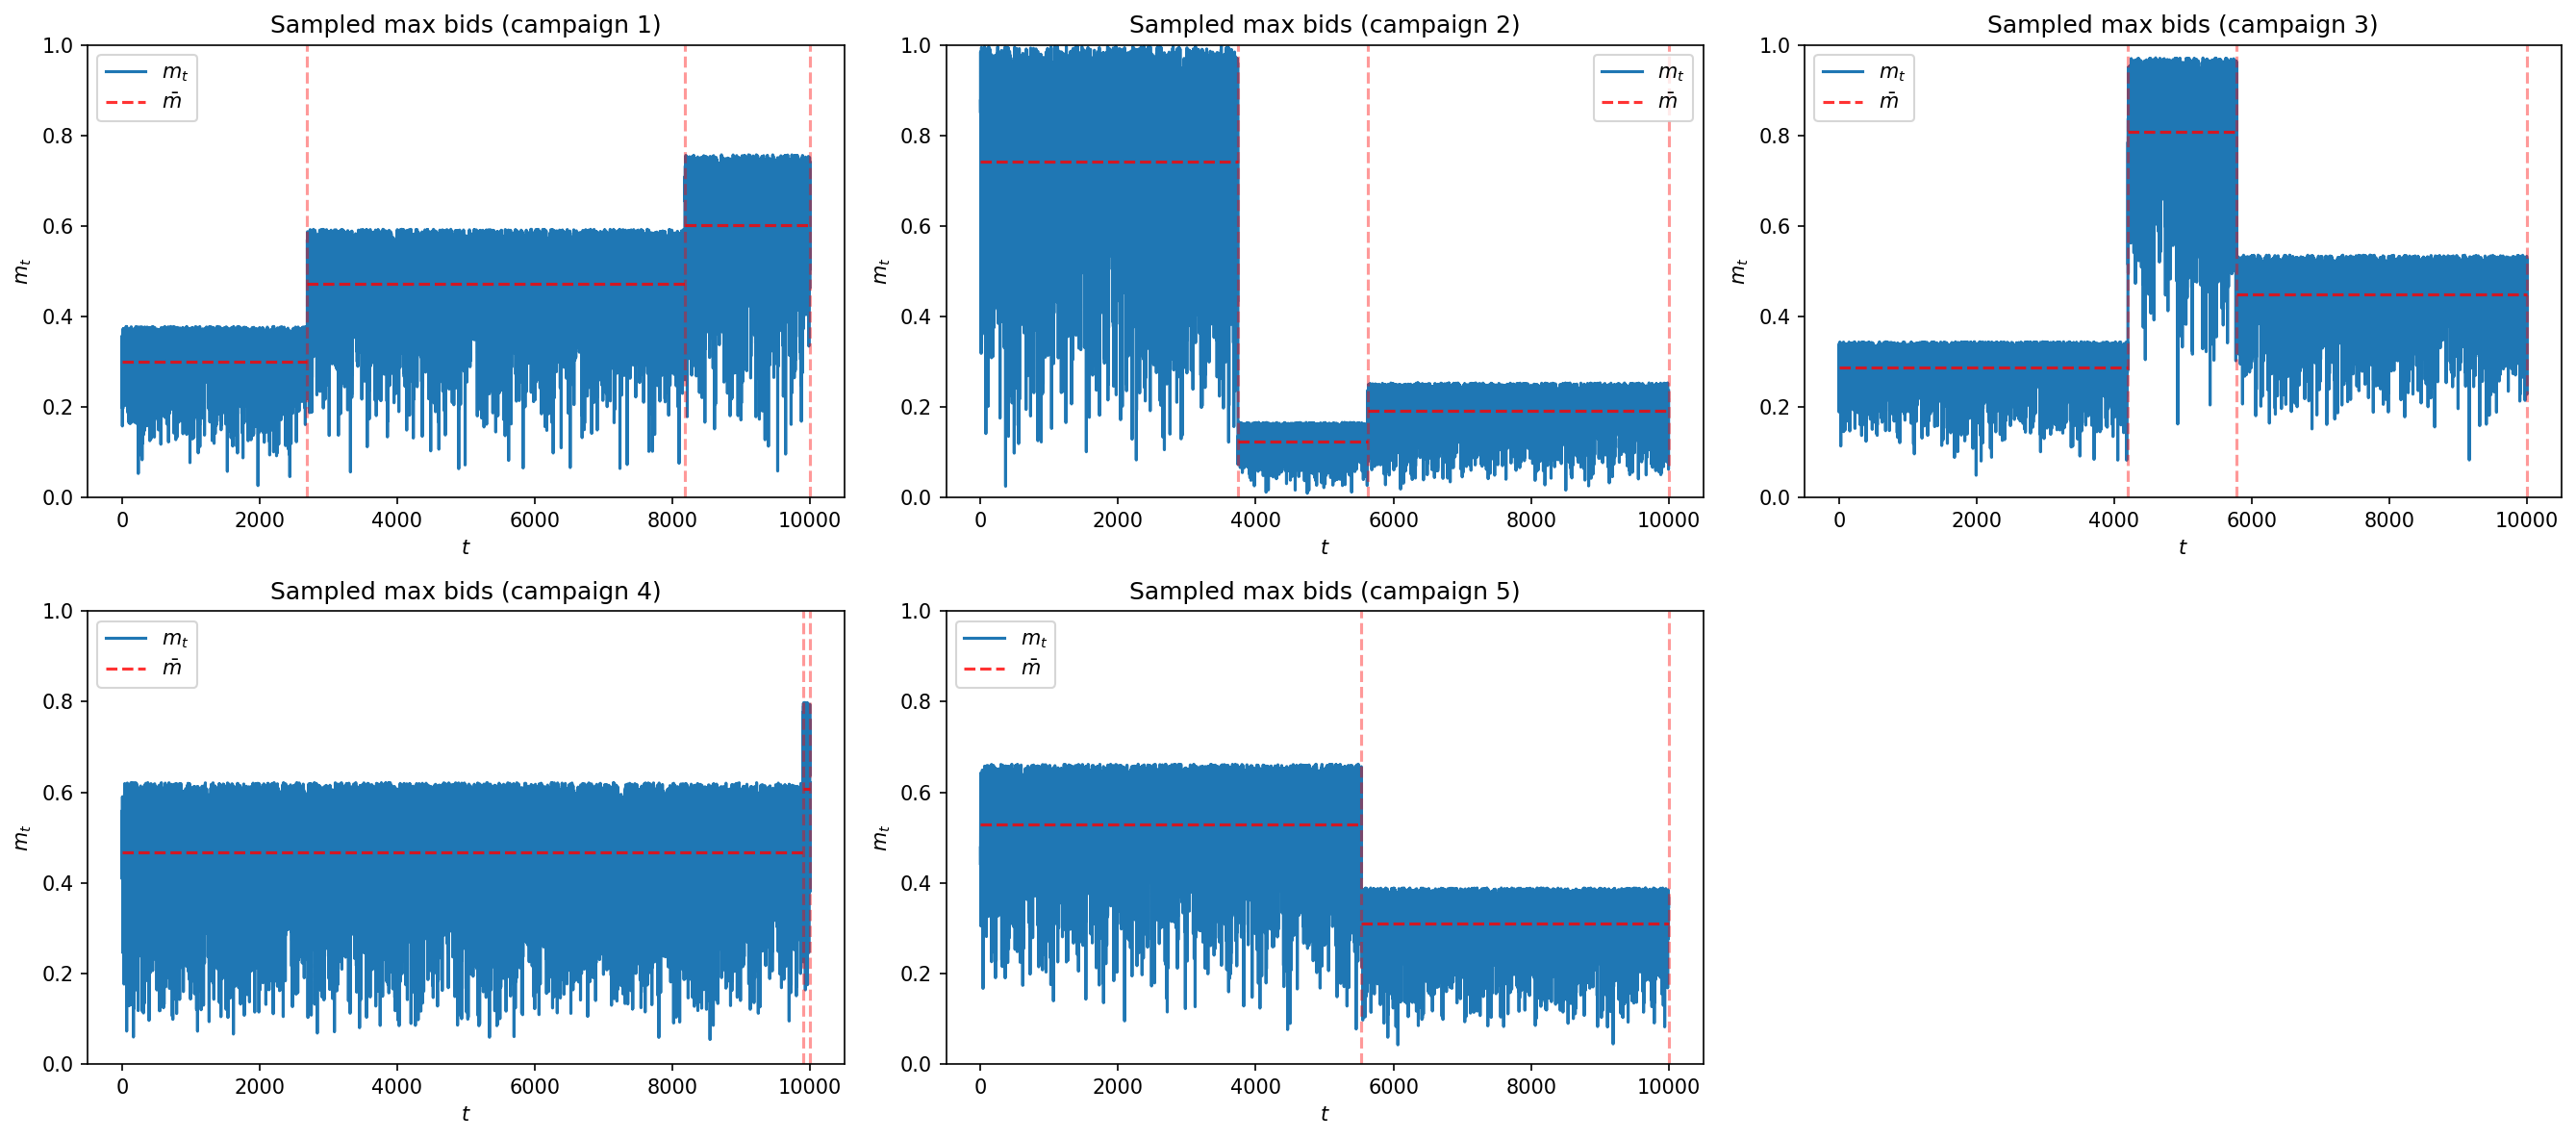
\includegraphics[width=0.7\textwidth]{figures/req4_max_bids_ts_with_changes.png}

    \vspace{-0.1cm}

    \footnotesize\begin{itemize}
        \item For each campaign $i$, independently sample the number of phases $\Upsilon_i \sim \mathrm{Unif}\{2, 3\}$ and then $\Upsilon_i-1$ change times uniformly in $[1,T]$
        
        \vspace{-0.1cm}
        
        \item Each phase has a different upper bound $u^{(i)}_p \sim \mathrm{Unif}(0, 1)$ on competitors' uniform bids
        
        \vspace{-0.1cm}
        
        \item Within a phase: competing bids $\sim \mathrm{Unif}(0, u^{(i)}_p)$, thus $m_p^{(i)} \sim \mathrm{Beta}(n_i,1)$ but \emph{rescaled by $u^{(i)}_p$} 

        \vspace{-0.05cm}

        $\implies$ closed-form win probabilities $\implies$ we \emph{can} write the same LP of the stochastic setting, per-phase
    \end{itemize}
\end{frame}

% ============================================================
% Clairvoyant LP -- piecewise stationary
% ============================================================
\begin{frame}{Clairvoyant: realistic baseline}
    \begin{itemize}
        \item Slightly non-stationary clairvoyant: the one implementing the \emph{best policy} in hindsight (defined in the exercise session)
        \item Actual best policy in a budget-constrained environment: deliberately do not bid at all in some phases, wait for later phases in which highest competing bids are lower instead.
        \item $\implies$ Completely unrealistic: no learner can foresee that a more favourable phase than the current one is coming in the future! 
        \begin{itemize}
            \item (See proof of lower bound for adversarial environment in the course slides)
        \end{itemize}
        \item Thus, we choose the clairvoyant \textbf{not as knowing all the changes in the highest competing bids in advance}, but \textbf{as being able to detect the changes instantaneously as they happen}
        \begin{itemize}
            \item In line with our learners: they "lose rounds" in detecting changes, or in trying to forget the past, or in adjusting against them
        \end{itemize}
    \end{itemize}
\end{frame}

\begin{frame}{Clairvoyant: a per-phase LP on each interval}
    Intersect the phases of all campaigns together and split rounds in a single \emph{joint} partition

    \vspace{0.2cm}

    \begin{block}{}
        A clairvoyant simply needs to solve a stationary LP for each phase in this joint partitioning!
        
        $\implies$ For each joint phase $p$: solve the same clairvoyant LP as in Requirement 2, with phase-specific win probabilities $\mathbb{P}^{(i)}_p(b \ge m)$
    \end{block}

    \vspace{0.8cm}

    \begin{alertblock}{Note:}
        $\rho$ stays the same across phases, it does not get updated!
    \end{alertblock}
\end{frame}


\begin{frame}{Clairvoyant: phase-wise $\gamma_s^\star$ over campaigns subsets}
    \centering
    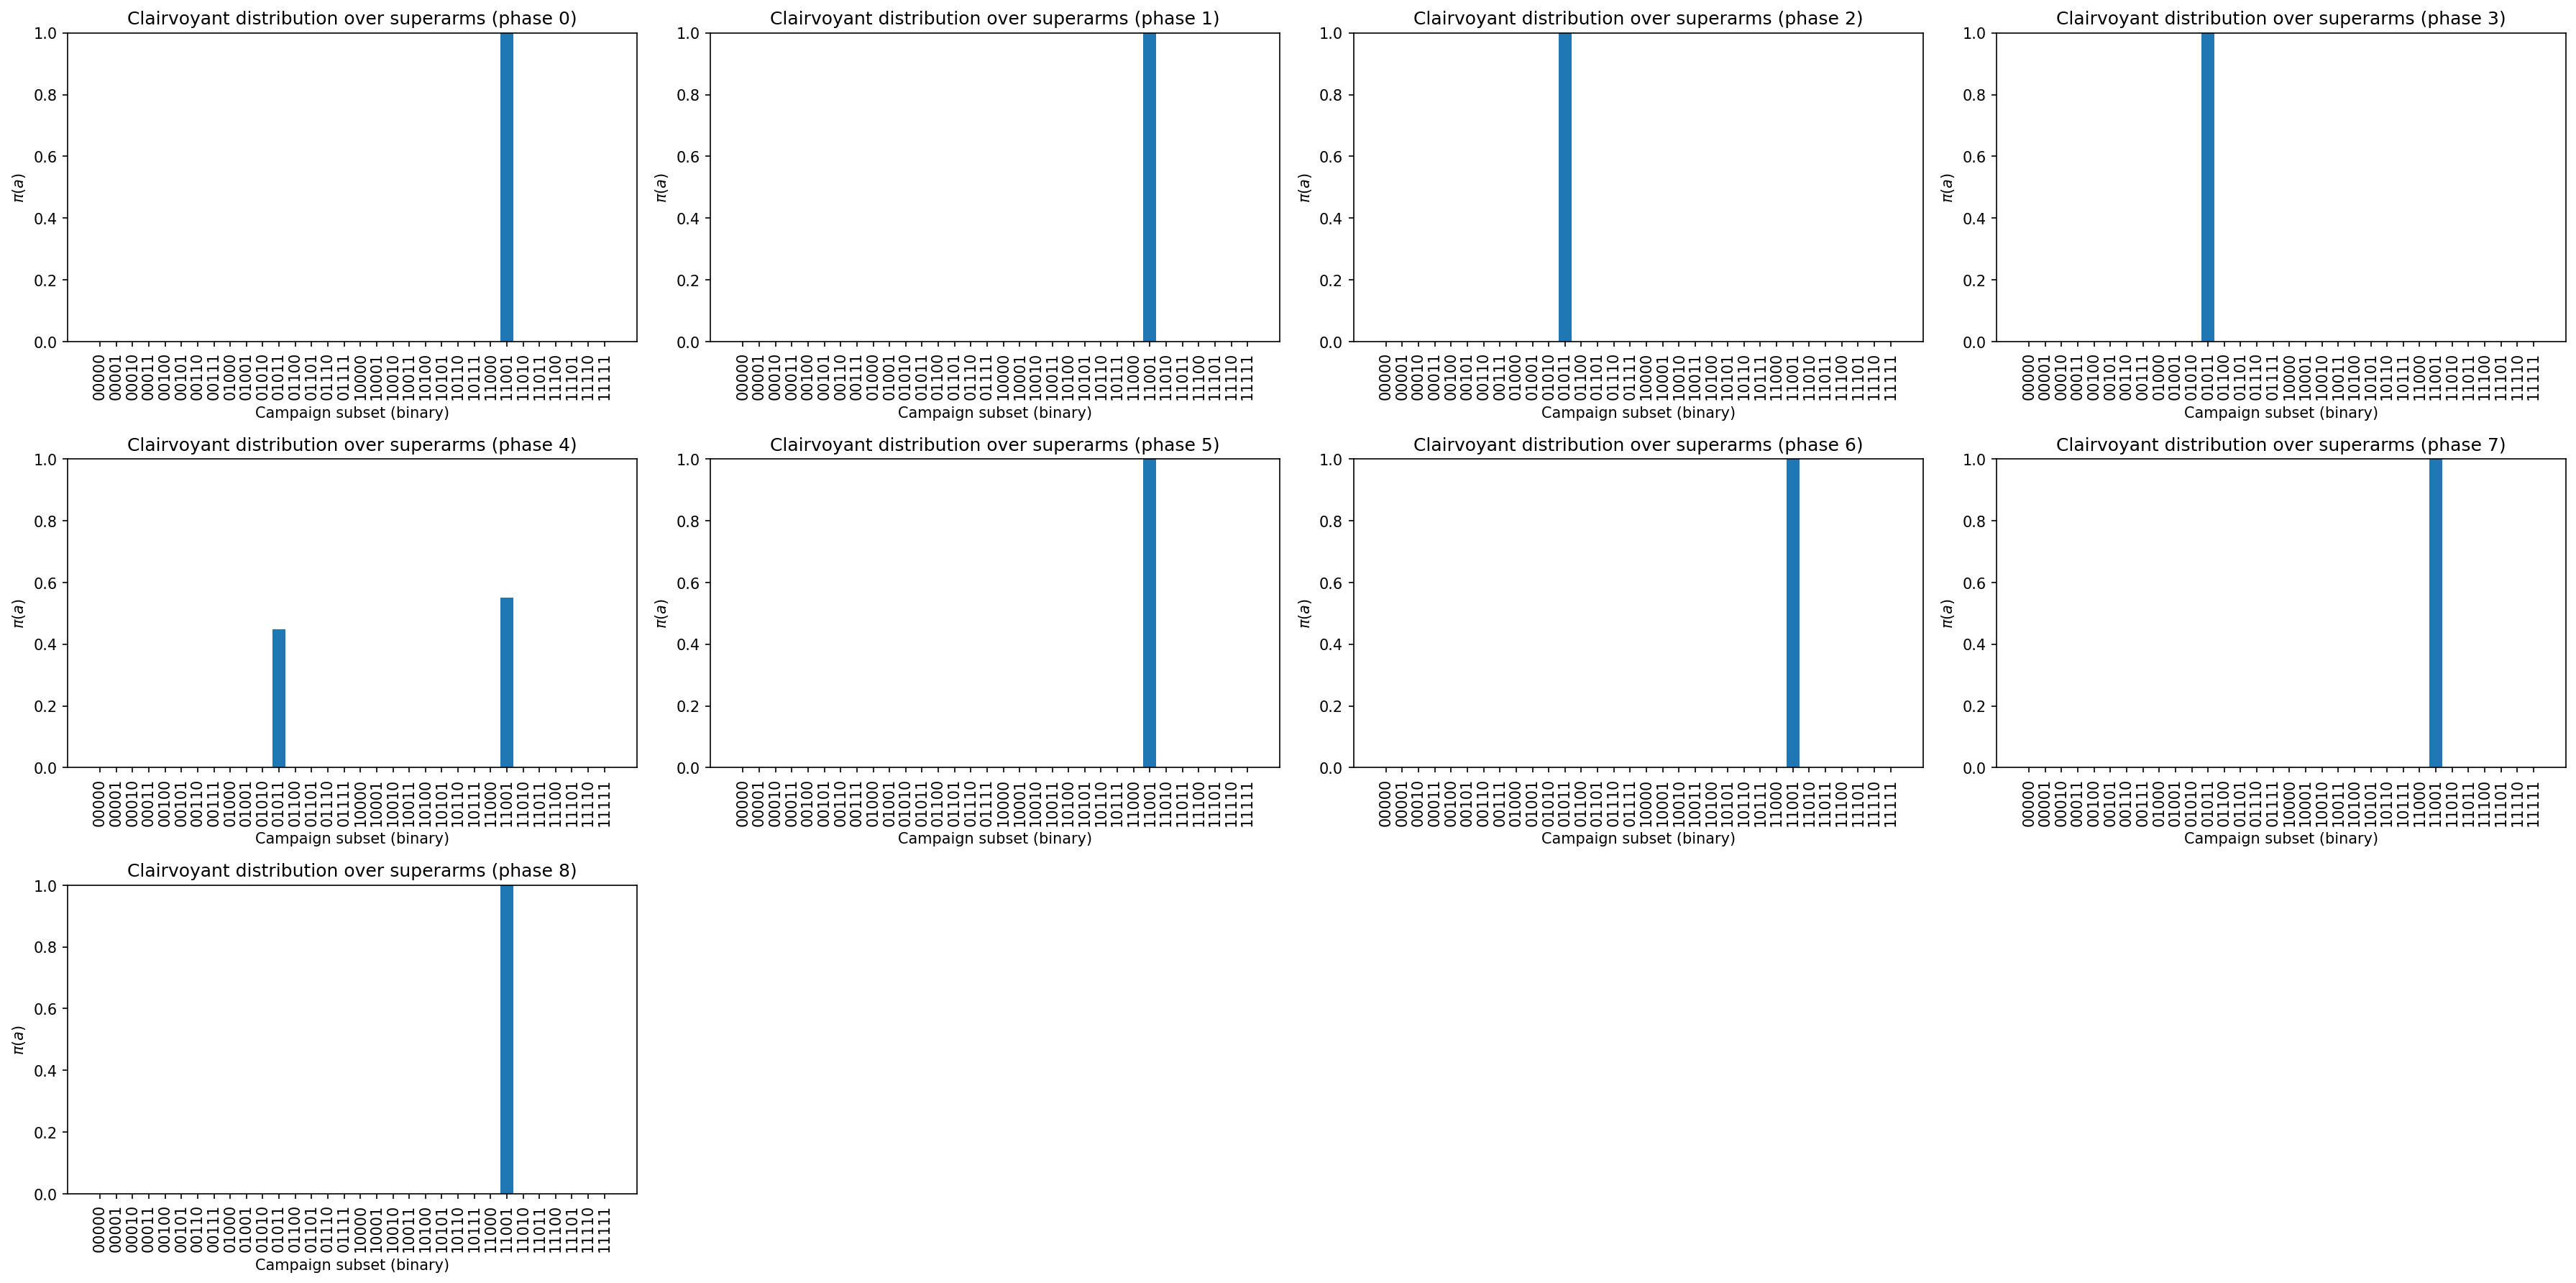
\includegraphics[width=0.8\textwidth]{figures/req4_clairvoyant_gamma_phases.png}\\
    \scriptsize
    Each phase has its own randomization policy over the subsets of campaigns: the policy changes because some campaigns become better/worse in different phases due to the competing bids being non-stationary.
\end{frame}

% ============================================================
% Sliding-window bidder
% ============================================================
\begin{frame}{Sliding-Window Combinatorial-UCB: recap}
    \begin{itemize}
        \item Maintain a \emph{window} of the samples played over the last $\tau$ rounds and the corresponding utilities/costs observed
        \item Confidence radius is computed on the window only: $r(b) = \sqrt{\frac{2 \log \tau}{N_\tau(b)}}$
        \item Theoretically optimal window size: $\tau = \sqrt{\frac{T\log T}{\Upsilon}}$, where $\Upsilon$ is the total amount of (\emph{joint}!) phases
        \begin{itemize}
            \item for unknown $\Upsilon$, set $\Upsilon = T \implies \tau = \sqrt{\log T}$
            \item $\tau \approx \sqrt{T}$ is also a good choice in practice: this is what we use
            \item we actually use $\tau \approx \sqrt{T \log T}$
        \end{itemize}
        
        \item Same underlying bidder as Combinatorial-UCB from Requirement 2
    \end{itemize}
\end{frame}

% ============================================================
% CUSUM bidder
% ============================================================
\begin{frame}{CUSUM Combinatorial-UCB: recap}
    Two phases:
    \begin{itemize}
        \item Estimation phase: build an estimator for the average utility/cost of each arm
        \begin{itemize}
            \item For each campaign, we set an exploration counter to a value $M$, and we keep exploring arms until all the counters reach $0$
            \item We try to select superarms that explore arms that require estimation for multiple campaigns at the same time
            \item At the same time, we do not bid on arms that we have already estimated to avoid wasting budget, since they may no longer be optimal
        \end{itemize}

        \item Detection phase: detect significant deviations from the estimated mean, which signal a phase change
        \begin{itemize}
            \item We compute the positive/negative deviation of the current utility/cost from the estimated means, "dampening" by a quantity $\varepsilon$
            \item We keep track of the positive/negative cumulative deviations from the estimates across multiple rounds
            \item We detect a change if either is larger than a threshold $h$
        \end{itemize}
    \end{itemize}
\end{frame}

\begin{frame}{CUSUM Combinatorial-UCB: recap}
    \begin{itemize}        
        \item Extra probability $\alpha$ of pure exploration per-round to detect changes in arms not being played
        \item Hyperparameters to be tuned: 
        \begin{itemize}
            \item $M$: Length of the estimation phase
            \item $\varepsilon$: "Dampening" factor, how much we expect a sample to deviate from the mean
            \item $h$: Threshold for detecting a change 
            \item $\alpha$: Probability of "pure" exploration per-round  
        \end{itemize}

        \item Again, same underlying bidder as Combinatorial-UCB from Requirement 2
    \end{itemize}
\end{frame}

\begin{frame}{CUSUM in action: detection traces}
    \centering
    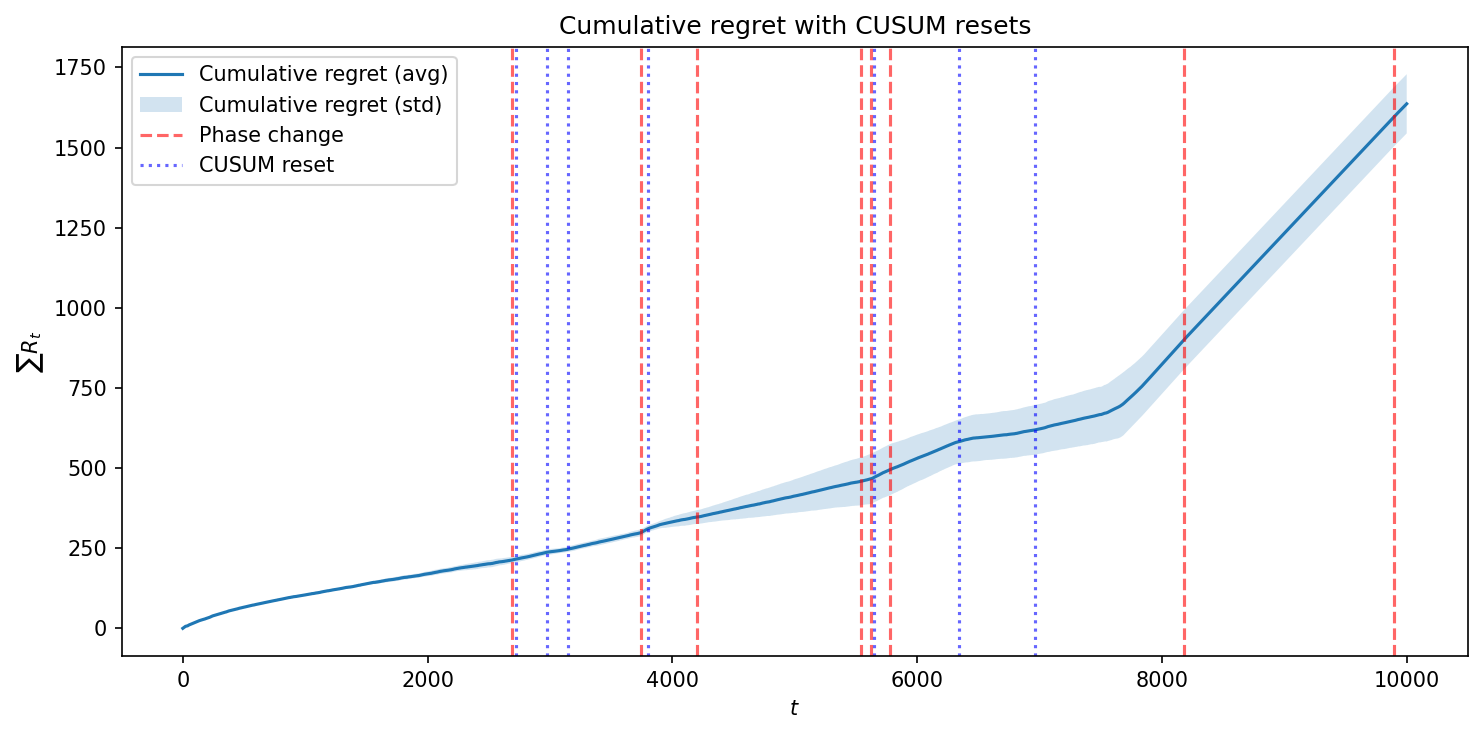
\includegraphics[width=0.75\textwidth]{figures/req4_cusum_resets.png}\\
    \scriptsize
    Joint phase change times (vertical \textcolor{red}{red} lines) and CUSUM reset times (vertical \textcolor{blue}{blue} lines) superimposed on the cumulative-regret curve. Regret can be convex/nonsmooth when changing phase, like the phase change right before round $4000$, or the ones right before round $6000$. A CUSUM reset time can lead to concavity and improvements in the regret, like in the two resets after round $6000$.
\end{frame}

% ============================================================
% Comparison
% ============================================================
\begin{frame}{Comparison: cumulative regret of the bidders}
    \centering
    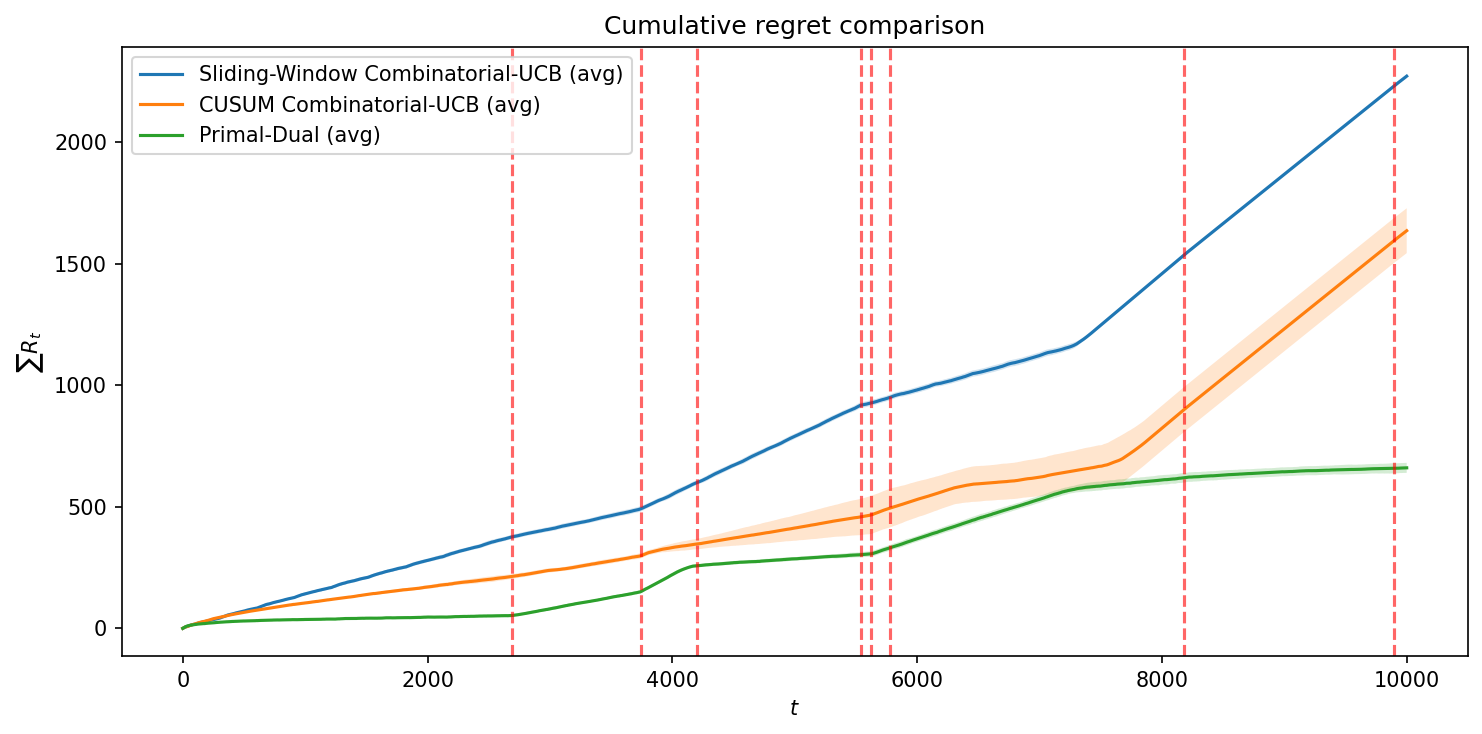
\includegraphics[width=0.75\textwidth]{figures/req4_regret_comparison.png}\\
    \scriptsize
    Unexpectedly, the primal-dual bidder remains the best, with CUSUM Combinatorial-UCB being a surprisingly close second, until it depletes the budget. Sliding-Window Combinatorial-UCB does a bit worse, maybe due to a suboptimal choice of the window size.
    Still, all regrets exhibit sublinear behavior until budget is depleted.
\end{frame}